\chapter{Discusión}
\label{cap:discusion}

El método de \textit{self-calibration} implementado, según los experimentos realizados en el capítulo \ref{cap:resultados}, permite su utilización tanto en conjunto de datos simulados como conjunto de datos reales. Sin embargo, considerando las métricas obtenidas y las imágenes mostradas se puede ver que este método implementado logra una calibración pero que no logra ser mayor pero a la vez no empeora en gran medida los datos para que el método de reconstrucción entregue un mal resultado. 

En el caso de los conjunto de datos simulados para \textit{long-baseline} se realiza la comparación de las imágenes obtenidas con los métodos de CLEAN y MEM, donde si bien en algunas iteraciones las imágenes resultantes no presentan un gran cambio visual, las métricas asociadas a estas dan un mejor indicio de la calidad de la imagen resultante. En la Figura \ref{fig:PSNR_plot} se puede ver el comportamiento de los valores de PSNR para el método de CLEAN y MEM, donde se puede ver que estos alcanzaron el mejor valor en distintas iteraciones, siendo la segunda imagen para el caso de \textit{self-calibration} con CLEAN y la quinta para el caso de \textit{self-calibration} con MEM. Esto quiere decir, según esta métrica, que en estas imagenes se logró disminuir en mayor medida el ruido de la imagen y/o aumentar el valor máximo de la imagen.   

\begin{figure}[!ht]
	\centering
	\captionsetup{justification=centering}
	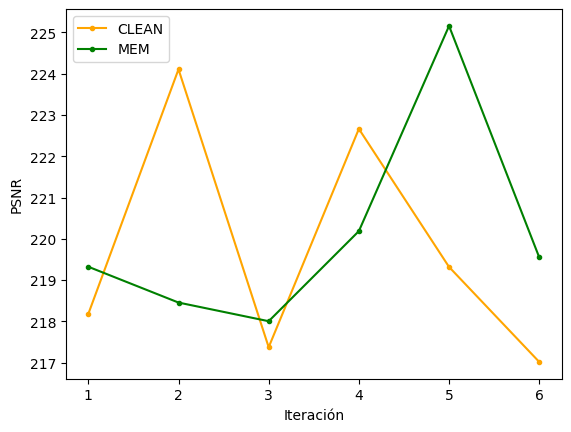
\includegraphics[scale=0.4]{images/PSNR_plot.png}
	\caption[Gráfico de PSNR para conjunto de datos simulado (\textit{long\_baseline})]{Gráfico de PSNR para conjunto de datos simulado (\textit{long-baseline}). Fuente: Elaboración propia}
	\label{fig:PSNR_plot}
\end{figure}

El comportamiento de la métrica NRMSE se puede observar en la Figura \ref{fig:NRMSE_long_sim}, donde se puede ver que según esta métrica las mejores imágenes se consiguen en la iteración 4 tanto para CLEAN y MEM. Si bien hay una discrepancia entre esta métrica y la anterior, hay que tener en cuenta que estas no están enfocadas en lo mismo, ya que si bien la anterior indicaba que la segunda y quinta iteración para CLEAN y MEM tienen la mejor relación señal/ruido, el NRMSE indica que la cuarta iteración para ambos métodos tienen una mayor similitud píxel a píxel con la imagen modelo.

\begin{figure}[!ht]
 \centering
  \subfloat[CLEAN]{
   \label{fig:CLEAN_NRMSE}
    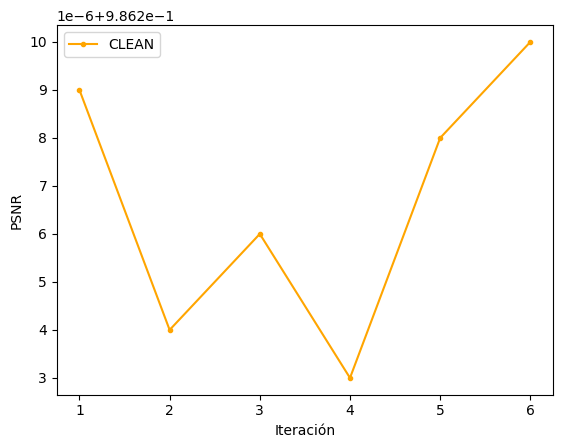
\includegraphics[width=0.45\textwidth]{images/NRMSE_CLEAN.png}}
  \subfloat[MEM]{
   \label{fig:MEM_NRMSE}
    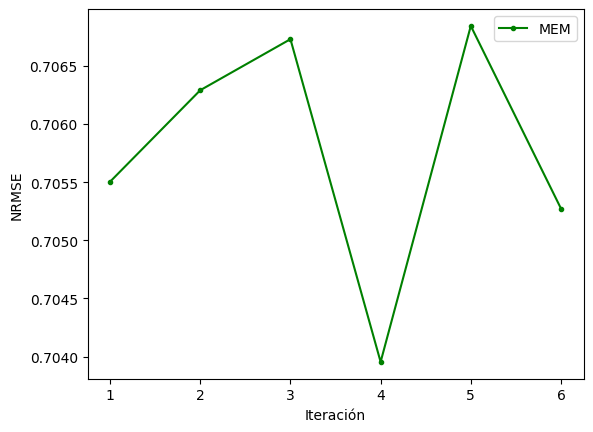
\includegraphics[width=0.48\textwidth]{images/NRMSE_MEM.png}}
 \caption[Gráfico para NRMSE para conjunto de datos simulados con método CLEAN y MEM (\textit{long-baseline})]{Gráfico para NRMSE para conjunto de datos simulados con método CLEAN y MEM (\textit{long-baseline}) Fuente: Elaboración propia.}
 \label{fig:NRMSE_long_sim}
\end{figure}

Si bien se realizaron diversas iteraciones para el conjunto de datos simulado para \textit{long-baseline} no necesariamente se deben realizar todas para obtener la mejor calidad de imagen, incluso se puede ver que la iteración final no da la mejor calidad de imagen. De esta manera, en la practica, se hubiera llegado hasta la segunda, cuarta o quinta iteración según el criterio del experto ya que fueron las que obtuvieron una mejor calidad de imagen. 

El conjunto de datos simulados en \textit{short-baseline}, al igual que el anterior, se realizó una comparación con las métricas de PSNR y MEM, donde se puede ver en la Figura \ref{fig:PSNR_short_sim} y Figura \ref{fig:NRMSE_short_sim} respectivamente. A diferencia de \textit{long-baseline} las métricas concuerdan por lo que la imagen final obtenida en la segunda iteración es la que tiene la mejor relación señal/ruido y a la vez tiene mayor similitud píxel a píxel con su imagen modelo. De esta manera el método de \textit{self-calibration} implementado es factible para aplicarse en \textit{short-baseline} junto a métodos como CLEAN y MEM. 

\begin{figure}[!ht]
 \centering
  \subfloat[CLEAN]{
   \label{fig:CLEAN_PSNR_short}
    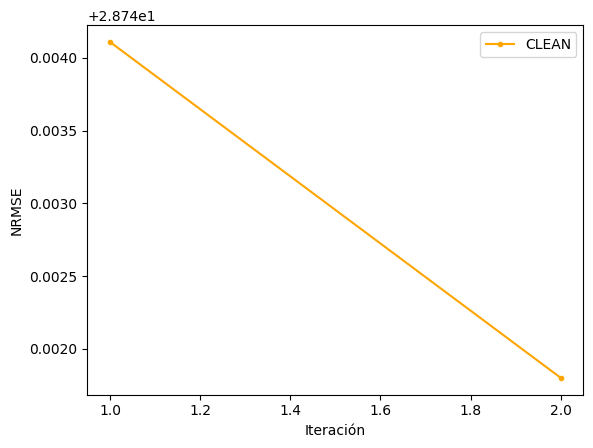
\includegraphics[width=0.45\textwidth]{images/PSNR_short_CLEAN.png}}
  \subfloat[MEM]{
   \label{fig:MEM_PSNR_short}
    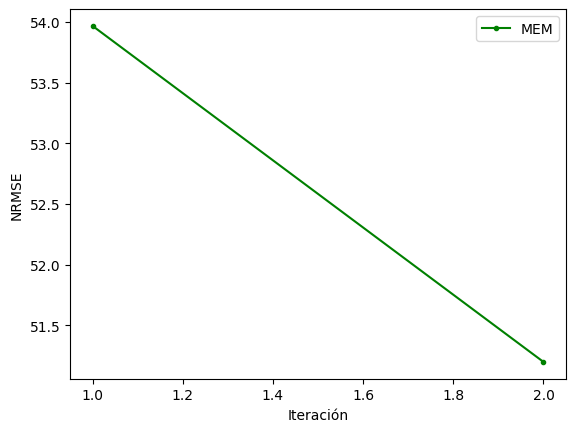
\includegraphics[width=0.45\textwidth]{images/PSNR_short_MEM.png}}
 \caption[Gráfico para PSNR para conjunto de datos simulados con método CLEAN y MEM (\textit{short-baseline})]{Gráfico para PSNR para conjunto de datos simulados con método CLEAN y MEM (\textit{short-baseline}) Fuente: Elaboración propia.}
 \label{fig:PSNR_short_sim}
\end{figure}

\begin{figure}[!ht]
 \centering
  \subfloat[CLEAN]{
   \label{fig:CLEAN_NRMSE_short}
    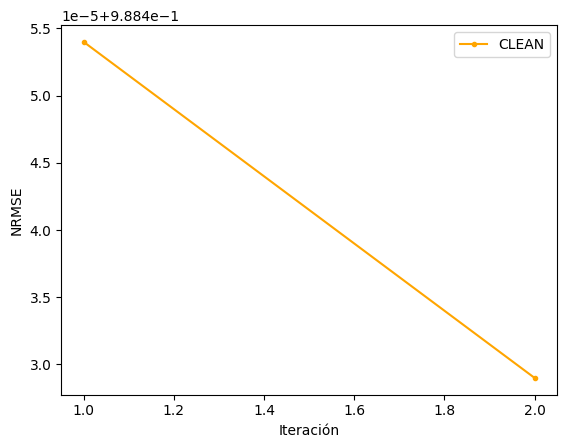
\includegraphics[width=0.45\textwidth]{images/NRMSE_short_CLEAN.png}}
  \subfloat[MEM]{
   \label{fig:MEM_NRMSE_short}
    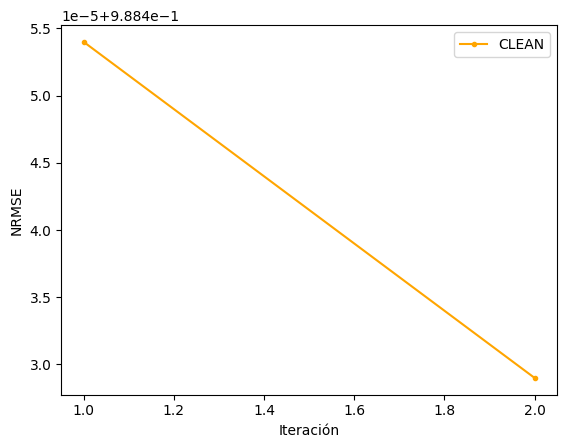
\includegraphics[width=0.45\textwidth]{images/NRMSE_short_CLEAN.png}}
 \caption[Gráfico para NRMSE para conjunto de datos simulados con método CLEAN y MEM (\textit{short-baseline})]{Gráfico para NRMSE para conjunto de datos simulados con método CLEAN y MEM (\textit{short-baseline}) Fuente: Elaboración propia.}
 \label{fig:NRMSE_short_sim}
\end{figure}

De esta manera, el método de \textit{self-calibration} realizado permite mejorar las visibilidades para el método de reconstrucción de imágenes a utilizar para un conjunto de datos simulado. Sin embargo, hay que tener en consideración que según los resultados obtenidos las diferencias de métricas (PSNR y NRMSE) tienden a ser a nivel de decimales y en ocasiones de unidades, por lo que a nivel visual puede no observarse una gran diferencia pero si el método es capaz de generar nuevas visibilidades sin empeorarlas lo suficiente para que la imagen resultante no sea reconocible. 

Si bien el método realizado es suficiente para el conjunto de datos simulados, también se realizan pruebas para un conjunto de datos real, por lo cual se realizaron experimentos con el conjunto HD163296 como se muestra en el capítulo \ref{cap:resultados}. Para el caso de \textit{long-baseline} se puede observar el comportamiento de la métrica PSNR para CLEAN y MEM en la Figura \ref{fig:PSNR_long_real}, donde se puede observar que para ambos casos la mejor iteración es la última aunque para el caso de CLEAN la tercera iteración es un caso aceptable ya que se acerca al valor de la última iteración. 

\begin{figure}[!ht]
 \centering
  \subfloat[CLEAN]{
   \label{fig:CLEAN_PSNR_long_real}
    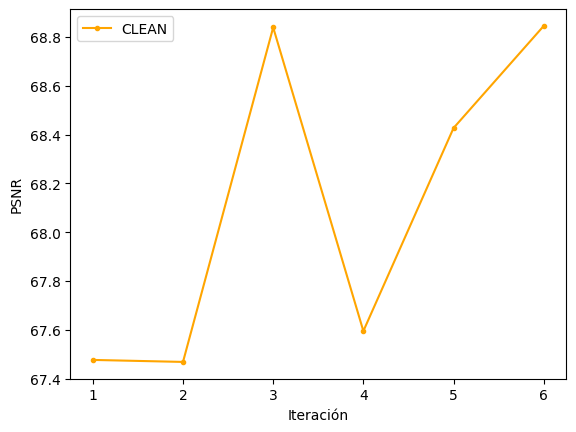
\includegraphics[width=0.45\textwidth]{images/PSNR_long_CLEAN.png}}
  \subfloat[MEM]{
   \label{fig:MEM_PSNR_long_real}
    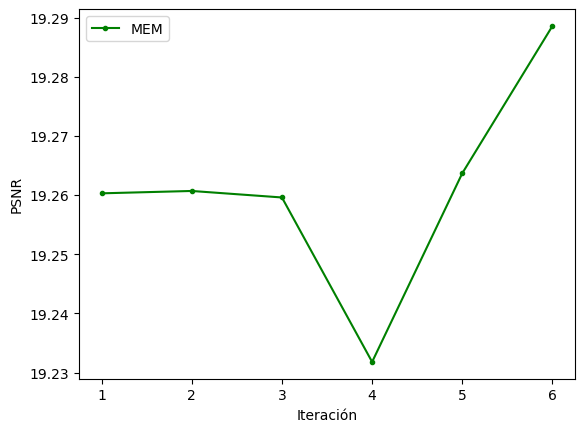
\includegraphics[width=0.45\textwidth]{images/PSNR_long_MEM.png}}
 \caption[Gráfico para PSNR para conjunto de datos HD163296 con método CLEAN y MEM (\textit{long-baseline})]{Gráfico para PSNR para conjunto de datos HD163296 con método CLEAN y MEM (\textit{long-baseline}) Fuente: Elaboración propia.}
 \label{fig:PSNR_long_real}
\end{figure}

En cuanto al NRMSE se puede observar su comportamiento para el conjunto de datos HD163296 en la Figura \ref{fig:NRMSE_long_real}. A través de esta se puede observar que para CLEAN la imagen que tiene un mayor grado de similitud con la modelo es la resultante de la tercera iteración, en cambio, para MEM es la resultante de la sexta iteración. Aunque algo a destacar es que los valores de NRMSE para MEM están muy alejados de 0 por lo que estas se encuentran en gran medida distanciadas de la imagen modelo, esto se puede observar ya que en las esquinas de la imagen (como por ejemplo en la figura \ref{fig:real_gpuvmem_p5_color}) se añade señal que no es parte de la imagen original.

\begin{figure}[!ht]
 \centering
  \subfloat[CLEAN]{
   \label{fig:CLEAN_NRMSE_long_real}
    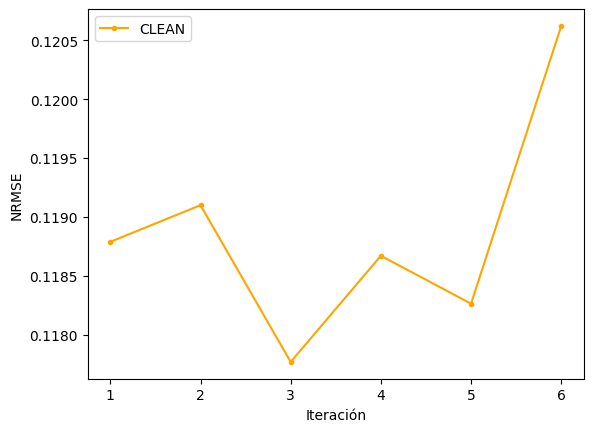
\includegraphics[width=0.45\textwidth]{images/NRMSE_long_CLEAN.png}}
  \subfloat[MEM]{
   \label{fig:MEM_NRMSE_long_real}
    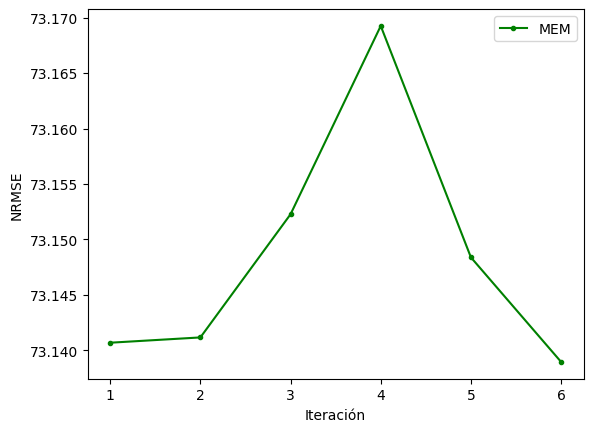
\includegraphics[width=0.45\textwidth]{images/NRMSE_long_MEM.png}}
 \caption[Gráfico para NRMSE para conjunto de datos HD163296 con método CLEAN y MEM (\textit{long-baseline})]{Gráfico para NRMSE para conjunto de datos HD163296 con método CLEAN y MEM (\textit{long-baseline}) Fuente: Elaboración propia.}
 \label{fig:NRMSE_long_real}
\end{figure}

En el caso de \textit{short-baseline} se tiene que los valores para el PSNR, tanto \textit{self-calibration} con el método CLEAN y MEM, se obtiene la Figura \ref{fig:PSNR_short_real}. Se puede observar que tanto para CLEAN y MEM, la mejor imagen se da en la segunda iteración debido a que esta tiene la mejor relación señal/ruido. Además, en la Figura \ref{fig:NRMSE_short_real} se puede observar que también la imagen resultante de la segunda iteración es la que tiene una mayor similitud con la imagen modelo. 

\begin{figure}[!ht]
 \centering
  \subfloat[CLEAN]{
   \label{fig:CLEAN_PSNR_short_real}
    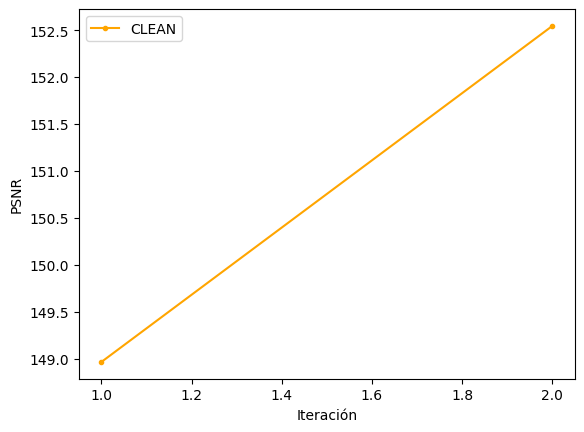
\includegraphics[width=0.45\textwidth]{images/PSNR_real_short_CLEAN.png}}
  \subfloat[MEM]{
   \label{fig:MEM_PSNR_short_real}
    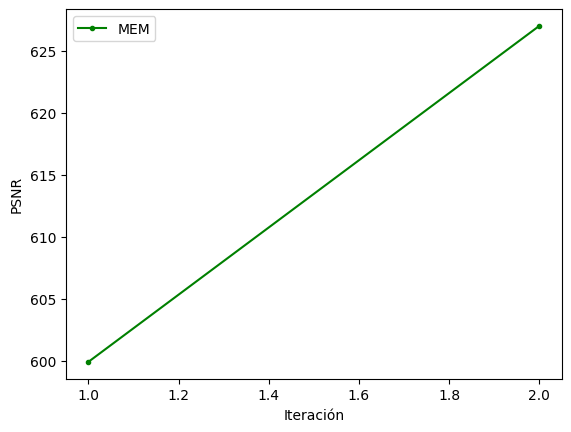
\includegraphics[width=0.45\textwidth]{images/PSNR_real_short_MEM.png}}
 \caption[Gráfico para PSNR para conjunto de datos HD163296 con método CLEAN y MEM (\textit{short-baseline})]{Gráfico para PSNR para conjunto de datos HD163296 con método CLEAN y MEM (\textit{short-baseline}) Fuente: Elaboración propia.}
 \label{fig:PSNR_short_real}
\end{figure}

\begin{figure}[!ht]
 \centering
  \subfloat[CLEAN]{
   \label{fig:CLEAN_NRMSE_short_real}
    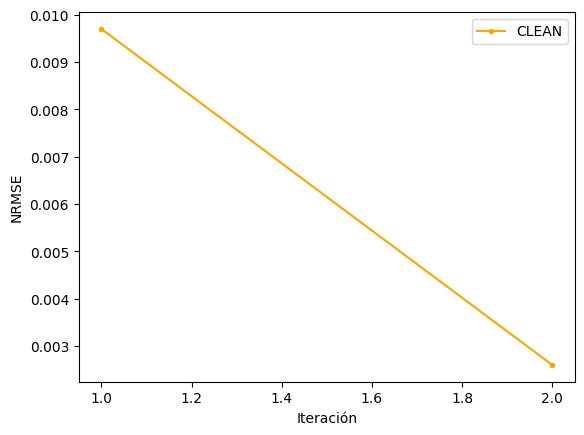
\includegraphics[width=0.45\textwidth]{images/NRMSE_real_short_CLEAN.png}}
  \subfloat[MEM]{
   \label{fig:MEM_NRMSE_short_real}
    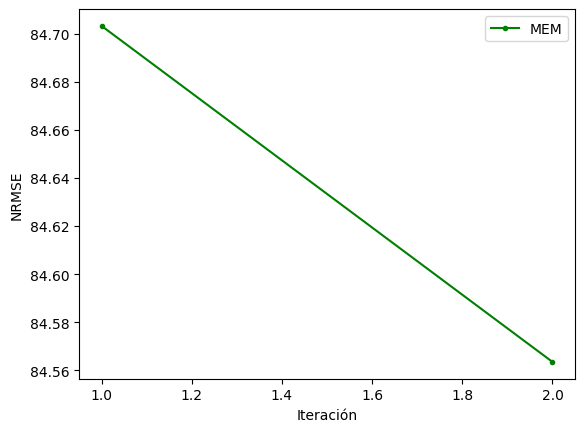
\includegraphics[width=0.45\textwidth]{images/NRMSE_real_short_MEM.png}}
 \caption[Gráfico para NRMSE para conjunto de datos HD163296 con método CLEAN y MEM (\textit{short-baseline})]{Gráfico para NRMSE para conjunto de datos HD163296 con método CLEAN y MEM (\textit{short-baseline}) Fuente: Elaboración propia.}
 \label{fig:NRMSE_short_real}
\end{figure}

El método de \textit{self-calibration} implementado muestra que puede trabajarse junto a otros métodos como \textit{CLEAN} y \textit{MEM} para conjunto de datos reales. Sin embargo, el método de \textit{self-calibration}, al igual que en los conjuntos simulados, en algunas iteraciones no logra un cambio visual en gran medida pero tampoco perjudica la imagen resultante final, si no que viendo las métricas planteadas se puede ver que \textit{self-calibration} es capaz de afectar el resultado en un par de decimales ya que gran parte de la calidad de la imagen resultante va en el método de reconstrucción. 

%Bispectrum
El \textit{bispectrum} desarrollado muestra que este es capaz de calcular, a través de la formula presentada en la sección \ref{subsec:bispectrum} del capitulo \ref{cap:marco}, las nuevas visibilidades \textit{bispectrum} que no son afectadas por el ruido de fase. Esto es demostrado al perturbar una fuente puntual y someterla a este método, obteniendo así las visibilidades iniciales sin perturbar. Por otro lado, el $\chi^{2}$ de esté método es capaz de retornar una imagen similar a la imagen sucia del conjunto de datos, lo que da un buen indicio para implementar un optimizador capaz de generar la mejor imagen según este método. 

Sin embargo, para verificar la implementación de un optimizador, es necesario saber si el $\chi^{2}$ es capaz de minimizar el valor de la función objetivo por lo que un optimizador para este método es factible. De esta manera la prueba realizada en el capitulo \ref{cap:resultados}, donde se escogen distintos valores de $\alpha$ para la ecuación $\chi^{2}(I - \alpha \nabla I)$, se observa en la figura \ref{fig:chi2_comp} el comportamiento del $\chi^{2}$ que va disminuyendo dependiendo del valor de $\alpha$. Sin embargo, esto se ve con claridad cuando los valores tienen una distancia entre ellos muy pequeña como es el caso de la figura \ref{fig:1e9} y \ref{fig:1e10} donde se puede ver una una relación inversa entre el valor de $\chi^{2}$ y de los $\alpha$. Aunque esto no ocurre para el caso cuando la distancia va aumentando, que es el caso de la figura \ref{fig:1e8} donde al final se puede ver que el valor de $\chi^{2}$ va en aumento, esto se puede deber a que con valores mas grande para la distancia entre $\alpha$ se está realizando un paso mas grande para buscar el mínimo y por ende se sale de la zona óptima de la función. 

